% DOCUMENT CLASS
%%%%%%%%%%%%%%%%%%%%%%%%%%%%%%%%%%%%%%%%%%%%%%%%%%%%%%%%%%%%%%%%%%%%%%%%%%%%%%%%%%%%%%%%%%%%%%%%%%%%%%

\documentclass[journal=jpcbfk,manuscript=article, articletitle=true]{achemso}
\SectionNumbersOn  % This is necessary to use section labels and referencing with ACS template.

% Single-spaced, two-column with PRL look and style (easy on the eyes)
%\documentclass[aps,pre,twocolumn,nofootinbib,superscriptaddress,linenumbers]{revtex4-1}

%\documentclass[aip, jcp, reprint]{revtex4-1}  % arxiv version
\pdfoutput=1  % for arxiv

% Double-spaced, one-column style (for submission/review/editing)
%\documentclass[aps,preprint,prl,superscriptaddress,showpacs]{revtex4}

%%%%%%%%%%%%%%%%%%%%%%%%%%%%%%%%%%%%%%%%%%%%%%%%%%%%%%%%%%%%%%%%%%%%%%%%%%%%%%%%%%%%%%%%%%%%%%%%%%%%%%
% PREAMBLE
%%%%%%%%%%%%%%%%%%%%%%%%%%%%%%%%%%%%%%%%%%%%%%%%%%%%%%%%%%%%%%%%%%%%%%%%%%%%%%%%%%%%%%%%%%%%%%%%%%%%%%

% FONT
% Change to a sans serif font for submission.  Comment out for arxiv.
%\usepackage{sourcesanspro}  % Comment out this and the next line for submission to ACS journal.
%\renewcommand*\familydefault{\sfdefault} %% Only if the base font of the document is to be sans serif
%
%\usepackage[T1]{fontenc}
%\usepackage[font=sf,justification=justified]{caption}
%\usepackage[font=sf]{floatrow}  % Disabled for ACS

% Rework captions to use sans serif font.  % Commented out for ACS
%\makeatletter	
%\renewcommand\@make@capt@title[2]{%
% \@ifx@empty\float@link{\@firstofone}{\expandafter\href\expandafter{\float@link}}%
%  {\sf\textbf{#1}}\sf\@caption@fignum@sep#2\quad
%}%
%\makeatother

\usepackage{amsmath}
\usepackage{amssymb}
\usepackage{graphicx}
\usepackage{caption}
%\usepackage{dcolumn}
\usepackage{boxedminipage}
\usepackage{verbatim}
\usepackage{booktabs}
\usepackage{subfigure}
\usepackage{listings}
\usepackage{color}

%\usepackage[colorlinks=true,citecolor=blue,linkcolor=blue]{hyperref}  % Commented out to remove colors per ACS requirements.

% The figures are in a figures/ subdirectory.
%\graphicspath{{../figures/}}

% italicized boldface for math (e.g. vectors)
\newcommand{\bfv}[1]{{\mbox{\boldmath{$#1$}}}}
% non-italicized boldface for math (e.g. matrices)
\newcommand{\bfm}[1]{{\bf #1}}          

% Pretty-printing of shell commands
\newcommand{\shellcmd}[1]{\\\ \texttt{\scriptsize\# #1}\\}

%\newcommand{\bfm}[1]{{\mbox{\boldmath{$#1$}}}}
%\newcommand{\bfm}[1]{{\bf #1}}
\newcommand{\expect}[1]{\left \langle #1 \right \rangle}                % <.> for denoting expectations over realizations of an experiment or thermal averages
\newcommand{\dhdl}{\frac{dH}{d\lambda}}
% vectors
\newcommand{\var}[1]{{\mathrm var}{(#1)}}
\newcommand{\x}{\bfv{x}}
\newcommand{\y}{\bfv{y}}
\newcommand{\f}{\bfv{f}}

\newcommand{\bfc}{\bfm{c}}
\newcommand{\hatf}{\hat{f}}

\newcommand{\bTheta}{\bfm{\Theta}}
\newcommand{\btheta}{\bfm{\theta}}
\newcommand{\bhatf}{\bfm{\hat{f}}}
\newcommand{\Cov}[1] {\mathrm{cov}\left( #1 \right)}
\newcommand{\Ept}[1] {{\mathrm E}\left[ #1 \right]}
\newcommand{\Eptk}[2] {{\mathrm E}_{#1}\left[ #2\right]}
\newcommand{\T}{\mathrm{T}}                                % T used in matrix transpose

%%%%%%%%%%%%%%%%%%%%%%%%%%%%%%%%%%%%%%%%%%%%%%%%%%%%%%%%%%%%%%%%%%%%%%%%%%%%%%%%
% DOCUMENT
%%%%%%%%%%%%%%%%%%%%%%%%%%%%%%%%%%%%%%%%%%%%%%%%%%%%%%%%%%%%%%%%%%%%%%%%%%%%%%%%


%%%%%%%%%%%%%%%%%%%%%%%%%%%%%%%%%%%%%%%%%%%%%%%%%%%%%%%%%%%%%%%%%%%%%%%%%%%%%%%%
% TITLE AND AUTHORS
%%%%%%%%%%%%%%%%%%%%%%%%%%%%%%%%%%%%%%%%%%%%%%%%%%%%%%%%%%%%%%%%%%%%%%%%%%%%%%%%

\title{Towards Automated Benchmarking of Atomistic Forcefields:\\
Neat Liquid Densities and Static Dielectric Constants from the ThermoML Data Archive}

\author{Kyle A. Beauchamp$^+$}
%\thanks{Corresponding author}  % Disabled for ACS
\email{kyle.beauchamp@choderalab.org}
\affiliation{Computational Biology Program, Sloan Kettering Institute, Memorial Sloan Kettering Cancer Center, New York, NY}

\author{Julie M. Behr$^+$}
%\email{julie.behr@choderalab.org}
\affiliation{Tri-Institutional Program in Computational Biology and Medicine, Weill Cornell Medical College, New York, NY}

\author{Ari\"{e}n S. Rustenburg}
%\email{bas.rustenburg@choderalab.org}
\affiliation{Graduate Program in Physiology, Biophysics, and Systems Biology, Weill Cornell Medical College, New York, NY}
 
 \author{Christopher I. Bayly}
% \email{bayly@eyesopen.com}
 \affiliation{OpenEye Scientific Software Inc., Santa Fe, NM}
 
 
 \author{Kenneth Kroenlein}
% \email{kenneth.kroenlein@nist.gov}
 \affiliation{Thermodynamics Research Center, NIST, Boulder, CO}
 
 \author{John D. Chodera}
%\thanks{Corresponding author}  % Disabled for ACS
 \email{john.chodera@choderalab.org}
 \affiliation{Computational Biology Program, Sloan Kettering Institute, Memorial Sloan Kettering Cancer Center, New York, NY}

\date{\today}

\includeonly{}

\begin{document}  % For ACS, had to move begin document to after the author info

%%%%%%%%%%%%%%%%%%%%%%%%%%%%%%%%%%%%%%%%%%%%%%%%%%%%%%%%%%%%%%%%%%%%%%%%%%%%%%%%
% ABSTRACT
%%%%%%%%%%%%%%%%%%%%%%%%%%%%%%%%%%%%%%%%%%%%%%%%%%%%%%%%%%%%%%%%%%%%%%%%%%%%%%%%

\clearpage

%\section{Abstract}
\begin{abstract}

Atomistic molecular simulations are a powerful way to make quantitative predictions, but the accuracy of these predictions depends entirely on the quality of the forcefield employed.
While experimental measurements of fundamental physical properties offer a straightforward approach for evaluating forcefield quality, the bulk of this information has been tied up in formats that are not machine-readable.
Compiling benchmark datasets of physical properties from non-machine-readable sources requires substantial human effort and is prone to the accumulation of human errors, hindering the development of reproducible benchmarks of forcefield accuracy.
Here, we examine the feasibility of benchmarking atomistic forcefields against the NIST ThermoML data archive of physicochemical measurements, which aggregates thousands of experimental measurements in a portable, machine-readable, self-annotating IUPAC-standard format. 
As a proof of concept, we present a detailed benchmark of the generalized Amber small molecule forcefield (GAFF) using the AM1-BCC charge model against experimental measurements (specifically bulk liquid densities and static dielectric constants at ambient pressure) automatically extracted from the archive, and discuss the extent of data available for use in larger scale (or continuously performed) benchmarks.  
The results of even this limited initial benchmark highlight a general problem with fixed-charge forcefields in the representation low dielectric environments such as those seen in binding cavities or biological membranes.  

%\emph{Keywords: molecular mechanics forcefields; forcefield parameterization; forcefield accuracy; forcefield validation; mass density; static dielectric constant; biomolecular simulation}

\end{abstract}

\maketitle

%%%%%%%%%%%%%%%%%%%%%%%%%%%%%%%%%%%%%%%%%%%%%%%%%%%%%%%%%%%%%%%%%%%%%%%%%%%%%%%%
% INTRODUCTION
%%%%%%%%%%%%%%%%%%%%%%%%%%%%%%%%%%%%%%%%%%%%%%%%%%%%%%%%%%%%%%%%%%%%%%%%%%%%%%%%

\section{Introduction}

Recent advances in hardware and software for molecular dynamics simulation now permit routine access to atomistic simulations at the 100 ns timescale and beyond~\cite{salomon2013routine}.
Leveraging these advances in combination with consumer GPU clusters, distributed computing, or custom hardware has brought microsecond and millisecond simulation timescales within reach of many laboratories.  
These dramatic advances in sampling, however, have revealed deficiencies in forcefields as a critical barrier to enabling truly predictive simulations of physical properties of biomolecular systems.  

Protein and water forcefields have been the subject of numerous benchmarks~\cite{lindorff2012systematic, beauchamp2012protein, best2008} and enhancements~\cite{li2011iterative, best2012optimization, Lindorff-Larsen2010}, with key outcomes including the ability to fold fast-folding proteins \cite{shaw2011, ensign2007heterogeneity, Voelz2010}, improved fidelity of water thermodynamic properties~\cite{horn2004}, and improved prediction of NMR observables.  
Although small molecule forcefields have also been the subject of benchmarks~\cite{caleman2011force, fischer2015properties, zhang2015force} and improvements~\cite{fennell2014fixed}, such work has typically focused on small perturbations to specific functional groups.  
For example, a recent study found that modified hydroxyl nonbonded parameters led to improved prediction of static dielectric constants and hydration free energies~\cite{fennell2014fixed}.
There are also outstanding questions of generalizability of these targeted perturbations; it is uncertain whether changes to the parameters for a specific chemical moiety will be compatible with seemingly unrelated improvements to other groups.
Addressing these questions requires establishing community agreement upon shared benchmarks that can be easily replicated among laboratories to test proposed forcefield enhancements and expanded as the body of experimental data grows.

A key barrier to establishing reproducible and extensible forcefield accuracy benchmarks is that many experimental datasets are heterogeneous, paywalled, and unavailable in machine-readable formats (although notable counterexamples exist, e.g.,~the PDB~\cite{Berman2000}, FreeSolv~\cite{freesolv}, and the BMRB~\cite{Ulrich2008}).  
While this inconvenience is relatively minor for benchmarking forcefield accuracy for a single target system (e.g.,~water), it becomes prohibitive for studies spanning relevant chemical spaces, such as forcefields intended to describe a large variety of druglike small organic molecules.  

In addition to inconvenience, the number and kind of human-induced errors that can corrupt hand-compiled benchmarks are legion.
A United States Geological Survey (USGS) case study examining the reporting and use of literature values of the aqueous solubility ($S_w$) and octanol-water partition coefficients ($K_{ow}$) for DDT and its persistent metabolite DDE provides remarkable insight into a variety of common errors~\cite{usgs-ddt-report}.
Secondary sources are often cited as primary sources---a phenomenon that occurred up to five levels deep in the case of DDT/DDE;
citations for data are often incorrect, misattributed to unrelated publications, or omitted altogether;
numerical data can be mistranscribed, transposed, or incorrectly converted among unit systems~\cite{usgs-ddt-report}.
In the case of DDT/DDE, these errors occur to such a degree that the authors note ``strings of erroneous data compose as much as 41--73 percent of the total data''~\cite{usgs-ddt-report}.
{\color{red} Given the number and importance of these measurements, the quality of physicochemical datasets of lesser importance may be suspect.}

To ameliorate problems of data archival, the NIST Thermodynamics Research Center (TRC) has developed an IUPAC standard XML-based format---ThermoML~\cite{frenkel2003thermoml, frenkel2006xml, chirico2013improvement}---for storing physicochemical measurements, uncertainties, and metadata.
%{\color{red}[KK: The conjugation on "data archival" feels odd; are you sure that's correct.]}
Manuscripts containing new experimental measurements submitted to several journals (J.~Chem.~Eng.~Data, J.~Chem.~Thermodyn., Fluid Phase Equilib., Thermochemica~Acta, and Int.~J.~Thermophys.) are guided through a data archival process that involves sanity checks, conversion to a standard machine-readable format, and archival at the TRC (\url{http://trc.nist.gov/ThermoML.html}).  

Here, we examine the ThermoML archive as a potential source for a reproducible, extensible accuracy benchmark of biomolecular forcefields.
As a proof of concept, we concentrate on two important physical property measurements easily computable in many simulation codes---neat liquid density and static dielectric constant measurements---with the goal of developing a standard benchmark for validating these properties in fixed-charge forcefields of drug-like molecules and biopolymer residue analogues.  
These two properties provide sensitive tests of forcefield accuracy that are nonetheless straightforward to calculate.  
Using these data, we evaluate the generalized Amber small molecule forcefield (GAFF)~\cite{gaff,gaff2} with the AM1-BCC charge model~\cite{am1bcc1,am1bcc2} and identify systematic biases to aid further forcefield refinement.




%%%%%%%%%%%%%%%%%%%%%%%%%%%%%%%%%%%%%%%%%%%%%%%%%%%%%%%%%%%%%%%%%%%%%%%%%%%%%%%%
% METHODS
%%%%%%%%%%%%%%%%%%%%%%%%%%%%%%%%%%%%%%%%%%%%%%%%%%%%%%%%%%%%%%%%%%%%%%%%%%%%%%%%

\section{Methods}
\label{section:methods}

\subsection{ThermoML Archive retrieval and processing}
\label{section:thermoml-archive-retrieval}

%{\color{red}[JDC: We should introduce this section by stating that, to facilitate automated benchmarking against available data, we first require an automated method for retrieving the data from the ThermoML Archive.  We first did this as described here, to explore the contents of the data, and then developed an automated tool to allow others to retrieve the dataset in an incremental and minimal-impact manner.]}
% KAB: we can document this feature on the Github page.  

A snapshot of the ThermoML Archive was obtained from the the NIST TRC on 8 Apr. 2015.
To explore the content of this archive, we created a Python (version 2.7.9) tool---ThermoPyL (\url{https://github.com/choderalab/ThermoPyL})---that formats the XML content into a spreadsheet-like format accessible via the Pandas (version 0.15.2) library.
This tool also contains a preliminary version of scripts for maintaining an up-to-date version of the ThermoML archive.
First, we obtained the XML schema (\url{http://media.iupac.org/namespaces/ThermoML/ThermoML.xsd}) defining the layout of the data.
This schema was converted into a Python object via PyXB 1.2.4 (\url{http://pyxb.sourceforge.net/}).
Finally, this schema was used to extract the data into Pandas~\cite{pandas} dataframes, and successive data filters described in Section~\ref{section:filtering-thermoml} were applied to explore the composition of the data.

\subsection{Simulation}
\label{section:simulation}

To enable automated accuracy benchmarking of physicochemical properties of neat liquids such as mass density and static dielectric constant, we developed a semi-automated pipeline for preparing simulations, running them on a standard computer cluster using a portable simulation package, and analyzing the resulting data.
All code for this procedure is available at  \url{https://github.com/choderalab/LiquidBenchmark}.
Below, we describe the operation of the various stages of this pipeline and their application to the benchmark reported here.

\subsubsection{Preparation}
\label{section:preparation}

Chemical names were parsed from the ThermoML extract and converted to both CAS and SMILES strings using cirpy (\url{https://github.com/mcs07/CIRpy}).  Smiles strings were converted into molecular structures using the OpenEye Python Toolkit version 2015-2-3 \cite{openeye}, as wrapped in openmoltools.  

Simulation boxes containing 1~000 molecules were constructed using PackMol version 14-225~\cite{martinez2009packmol} wrapped in the Python automation library openmoltools  (\url{http://github.com/choderalab/openmoltools/}).
In order to ensure stable automated equilibration, PackMol box volumes were chosen to accommodate twice volume of the enclosed atoms, with atomic radii estimated as 1.06 \AA\ and 1.53 \AA\ for hydrogens and nonhydrogens, respectively.  

For this illustrative benchmark, we utilized the generalized Amber small molecule forcefield (GAFF)~\cite{gaff,gaff2} with the AM1-BCC charge model~\cite{am1bcc1,am1bcc2}, which we shall refer to as the GAFF/AM1-BCC forcefield.
%{\color{red}[JDC: Missing statement about how the GAFF forcefield parameterization was applied (via antechamber?) here.]}
% this statement is at the end of the next paragraph. 

Canonical AM1-BCC~\cite{am1bcc1,am1bcc2, velez2014time} charges were generated with the OpenEye Python Toolkit version 2015-2-3 \cite{openeye}, using the {\tt oequacpac.OEAssignPartialCharges} module with the {\tt OECharges\_AM1BCCSym} option, which utilizes a conformational expansion procedure (using {\tt oeomega.OEOmega} \cite{hawkins2012conformer}) prior to charge fitting to minimize artifacts from intramolecular contacts.  
The {\tt OEOmega} selected conformer was then processed using {\tt antechamber} (with {\tt parmchk2}) and {\tt tleap} in AmberTools~14~\cite{amber14} to produce Amber-format {\tt prmtop} and {\tt inpcrd} files, which were then read into OpenMM to perform molecular simulations using the {\tt simtk.openmm.app} module.

The simulations reported here used libraries openmoltools~0.6.4, OpenMM~6.3~\cite{eastman2012openmm}, and MDTraj~1.3~\cite{mcgibbon2014mdtraj}.  
Exact commands to install various dependencies can be found in section S1.1.

\subsubsection{Equilibration and production}
\label{section:production}

All simulations were performed using OpenMM~6.3~\cite{eastman2012openmm}.
Simulation boxes were first minimized using the L-BFGS algorithm~\cite{liu1989limited} using the {\tt LocalEnergyMinimizer} default parameters and subsequently equilibrated for $10^7$ steps with an equilibration timestep of 0.4 fs and a collision rate of 5 ps$^{-1}$.  
Production simulations employed a Langevin Leapfrog integrator~\cite{izaguirre-sweet-pande:psb:2010:langevin-leapfrog} with collision rate 1 ps$^{-1}$ and a 1~fs timestep, as we found that timesteps of 2~fs or greater led to a significant timestep dependence in computed equilibrium densities (Fig.~\ref{figure:timestep}).  

Equilibration and production simulations utilized a Metropolis Monte Carlo barostat with a control pressure of 1 atm (101.325 kPa), utilizing molecular scaling and automated step size adjustment during equilibration, with volume moves attempted every 25 steps.  
The particle mesh Ewald (PME) method with conducting boundary conditions~\cite{Darden1993} was used with a long-range cutoff of 0.95~nm, and a long-range isotropic dispersion correction was employed to correct for the truncation of Lennard-Jones interactions outside the 0.95~nm cutoff.
PME grid and spline parameters were automatically selected using the default settings in OpenMM 6.3 for the CUDA platform~\cite{eastman2012openmm}, which was operated in default mixed-precision mode.
Instantaneous densities were stored every 250~fs, while trajectory snapshots were stored every 5~ps.  

{\bf Automatic termination criteria.}
Production simulations were continued until automatic analysis showed standard errors in densities were less than 2$\times$10$^{-4}$ g/cm$^{3}$.
Automatic analysis of the production simulation data was run every 1 ns of simulation time, and utilized the {\tt detectEquilibration} method \cite{equilibrationdetection} in the timeseries module of pymbar 2.1~\cite{shirts2008statistically} to automatically discard the initial portion of the production simulation containing strong far-from-equilibrium configurations.
This procedure selects the equilibration endpoint $T_\mathrm{eq}$ by maximizing the number of effectively uncorrelated samples in the remainder of the production simulation, $N_\mathrm{eff} = (T - T_\mathrm{equil}) / g$, with $T$ the total simulation length.
The statistical inefficiency $g$ was determined by autocorrelation analysis using the fast adaptive statistical inefficiency computation method as implemented in the {\tt timeseries.computeStatisticalInefficiency} method of pymbar 2.1 (where the algorithm is described in~\cite{chodera2007}).
This approach is essentially the same as the fixed-width procedure described by eq. 7.12 of ref. \cite{brooks2011handbook}, with $n^*$ equal to 4000 and the sequential testing correction ($n^{-1}$ term) ignored due to the large value of $n$.

Statistical errors in estimated average density $\left< \rho \right>$ were computed by the Markov chain standard error (MCSE)
\begin{eqnarray}
\delta \rho &\approx& \frac{\mathsf{std}(\rho)}{\sqrt{N_\mathrm{eff}}} \label{equation:density-standard-error}
\end{eqnarray}
where $\mathsf(\rho)$ is the sample standard deviation of the density and $N_\mathrm{eff}$ is the number of effectively uncorrelated samples.  

Using this adaptive protocol, we found starting trajectory lengths of $12000$ $(8000, 16000)$ density frames (250 fs each), discarded regions of $28$  $(0, 460)$ density frames, and statistical inefficiencies of $20$ $(15, 28)$ density frames; reported numbers indicate (median, (25\% quartile, 75\% quartile)).  

\subsection{Timings}

The wall time required for a given simulation depends on the number of atoms in the simulation system (3~000--29~000 atoms), the GPU used (GTX 680 or GTX Titan), and the time required for automated termination.  
For butyl acrylate (21~000 atoms) on a GTX Titan, the wall-clock performance is approximately 80 ns / day.  Using 80 ns / day with approximately 3 ns of production simulation corresponds to 1 hour for the production segment of the simulation and 3 hours for the fixed equilibration portion of $10^7$ steps.  

\subsubsection{Data analysis and statistical error estimation}

Trajectory analysis was performed using OpenMM~6.3~\cite{eastman2012openmm} and MDTraj~1.3~\cite{mcgibbon2014mdtraj}.  

{\bf Mass density.}
Mass density $\rho$ was computed via the relation,
\begin{eqnarray}
\rho = \left\langle \frac{M}{V} \right\rangle \label{equation:mass-density} ,
 \end{eqnarray}
where $M$ is the total mass of all particles in the system and $V$ is the instantaneous volume of the simulation box.

{\bf Static dielectric constants.}
Static dielectric constants were calculated using the dipole fluctuation approach appropriate for PME with conducting (``tin-foil'') boundary conditions~\cite{horn2004, neumann1983dipole}, with the total system box dipole $\mu$ computed from trajectory snapshots using MDTraj 1.3~\cite{mcgibbon2014mdtraj}.
\begin{eqnarray}
\epsilon = 1 + \beta \frac{4\pi}{3} \frac{\langle \mu \cdot \mu \rangle - \langle \mu \rangle \cdot \langle \mu \rangle}{\langle V \rangle} \label{equation:dielectric_calculation}
\end{eqnarray}
where $\beta \equiv 1 / k_\textnormal{B} T$ is the inverse temperature.

{\bf Computation of expectations.}
Expectations were estimated by computing sample means over the production simulation after discarding the initial far-from-equilibrium portion to equilibration (as described in {\bf Automatic termination criteria} above).

{\bf Statistical uncertainties.}
For density uncertainties, the Markov chain standard error (MCSE) was estimated using Eq.~\ref{equation:density-standard-error}.
For dielectric uncertainties, in order to avoid the complexities of computing and propagating correlated errors in Eq.~\ref{equation:dielectric_calculation}, a bootstrap procedure was employed: the portion of the production simulation not discarded to equilibration was used as input to a circular block bootstrapping procedure \cite{sheppard_2015_15681} with block sizes automatically selected to maximize the error \cite{flyvbjerg1989error}.

\subsubsection{Code availability}

All code to perform data analysis and create figures for this work, as well as all intermediate data (except configurational trajectories, due to their large size), is available at \url{https://github.com/choderalab/LiquidBenchmark}.  

%%%%%%%%%%%%%%%%%%%%%%%%%%%%%%%%%%%%%%%%%%%%%%%%%%%%%%%%%%%%%%%%%%%%%%%%%%%%%%%%
% RESULTS
%%%%%%%%%%%%%%%%%%%%%%%%%%%%%%%%%%%%%%%%%%%%%%%%%%%%%%%%%%%%%%%%%%%%%%%%%%%%%%%%

\section{Results}

\subsection{Extracting neat liquid measurements from the NIST TRC ThermoML Archive}
\label{section:filtering-thermoml}

As described in Section~\ref{section:thermoml-archive-retrieval}, we retrieved a copy of the ThermoML Archive and performed a number of sequential filtering steps to produce an ThermoML extract relevant for benchmarking forcefields describing small organic molecules.  
As our aim is to explore neat liquid data with functional groups relevant to biopolymers and drug-like molecules, we applied the following ordered filters, starting with all data containing density or static dielectric constants: 
\begin{enumerate}
 \item The measured sample contains only a single component (e.g.,~no binary mixtures)
 \item The molecule contains only druglike elements (defined here as H, N, C, O, S, P, F, Cl, Br)
 \item The molecule has $\le$ 10 non-hydrogen atoms
 \item The measurement was performed in a biophysically relevant temperature range $(270 \le T$ [K] $\le 330)$
 \item The measurement was performed at ambient pressure $(100 \le P$ [kPa]  $\le 102)$
 \item Only measurements in liquid phase were retained
 \item The temperature and pressure were rounded to nearby values (as described below), averaging all measurements within each group of like conditions
 \item Only conditions (molecule, temperature, pressure) for which \emph{both} density and dielectric constants were available were retained
\end{enumerate}
The temperature and pressure rounding step was motivated by common data reporting variations; for example, an experiment performed at the freezing temperature of water and ambient pressure might be entered as either 101.325~kPa or 100~kPa, with a temperature of either 273~K or 273.15~K.  
Therefore all pressures within the range [kPa] $(100 \le P \le 102)$ were rounded to exactly 1 atm (101.325 kPa).  
Temperatures were rounded to one decimal place in K. 

The application of these filters (Table~\ref{table:ThermoMLSummary}) leaves 246 conditions---where a \emph{condition} here indicates a (molecule, temperature, pressure) tuple---for which both density and dielectric data are available.  
The functional groups present in the resulting dataset are summarized in Table~\ref{table:FunctionalGroups}; see Section~\ref{section:thermoml-archive-retrieval} for further description of the software pipeline used.  

%%%%%%%%%%%%%%%%%%%%%%%%%%%%%%%%%%%%%%%%%%%%%%%%%%%%%%%%%%%%%%%%%%%%%%%%%%%%%%%%
% TABLE: DENSITY AND STATIC DIELECTRIC
%%%%%%%%%%%%%%%%%%%%%%%%%%%%%%%%%%%%%%%%%%%%%%%%%%%%%%%%%%%%%%%%%%%%%%%%%%%%%%%%

\begin{table}
\begin{tabular}{lrr}
\hline
 &  \multicolumn{2}{c}{\bf Number of measurements remaining} \\ \cline{2-3}
{\bf Filter step} &  {\bf Mass density} &  {\bf Static dielectric} \\ 
\hline
1.  Single Component   &               136212 &                                     1651 \\
2.  Druglike Elements  &               125953 &                                     1651 \\
3.  Heavy Atoms        &                71595 &                                     1569 \\
4.  Temperature        &                38821 &                                      964 \\
5.  Pressure           &                14103 &                                      461 \\
6.  Liquid state       &                14033 &                                      461 \\
7.  Aggregate T, P     &                 3592 &                                      432 \\
8.  Density+Dielectric &                  246 &                                      246 \\

\hline
\end{tabular}
\caption{{\bf Successive filtration of the ThermoML Archive.}
A set of successive filters were applied to all measurements in the ThermoML Archive that contained either mass density or static dielectric constant measurements.
Each column reports the number of measurements remaining after successive application of the corresponding filtration step.  
The 246 final measurements correspond to 45 unique molecules measured at several temperature conditions.  
}
\label{table:ThermoMLSummary}
\end{table}

\begin{table}
\begin{tabular}{lr}
\toprule
{\bf Functional Group} &    {\bf Occurrences} \\
\midrule
1,2-aminoalcohol                                    &   4 \\
1,2-diol                                            &   3 \\
alkene                                              &   3 \\
aromatic compound                                   &   1 \\
carbonic acid diester                               &   2 \\
carboxylic acid ester                               &   4 \\
dialkyl ether                                       &   7 \\
heterocyclic compound                               &   3 \\
ketone                                              &   3 \\
lactone                                             &   1 \\
primary alcohol                                     &  19 \\
primary aliphatic amine (alkylamine)                &   2 \\
primary amine                                       &   2 \\
secondary alcohol                                   &   4 \\
secondary aliphatic amine (dialkylamine)            &   2 \\
secondary aliphatic/aromatic amine (alkylarylamine) &   1 \\
secondary amine                                     &   3 \\
sulfone                                             &   1 \\
sulfoxide                                           &   1 \\
tertiary aliphatic amine (trialkylamine)            &   3 \\
tertiary amine                                      &   3 \\
\bottomrule
\end{tabular}
\caption{{\bf Functional groups present in filtered dataset.}  
The filtered ThermoML dataset contained 246 distinct (molecule, temperature, pressure) conditions, spanning 45 unique compounds.
The functional groups represented in these compounds (as identified by the program {\tt checkmol} v0.5~\cite{haider2010functionality}) is summarized here.
}
\label{table:FunctionalGroups}
\end{table}

%%%%%%%%%%%%%%%%%%%%%%%%%%%%%%%%%%%%%%%%%%%%%%%%%%%%%%%%%%%%%%%%%%%%%%%%%%%%%%%%
% DENSITY
%%%%%%%%%%%%%%%%%%%%%%%%%%%%%%%%%%%%%%%%%%%%%%%%%%%%%%%%%%%%%%%%%%%%%%%%%%%%%%%%

\subsection{Benchmarking GAFF/AM1-BCC against the ThermoML Archive}

\subsubsection{Mass density}

Mass densities of bulk liquids have been widely used for parameterizing and testing forcefields, particularly the Lennard-Jones parameters representing dispersive and repulsive interactions~\cite{jorgensen1983comparison, jorgensen1984optimized}.
We therefore used the present ThermoML extract as a benchmark of the GAFF/AM1-BCC forcefield (Fig.~\ref{figure:Density}).  

{\bf Overall accuracy.}
Overall, the densities show reasonable accuracy, with a root-mean square (RMS) relative error over all measurements of (3.0$\pm$0.1)\%, especially encouraging given that this forcefield was not designed with the intention of modeling bulk liquid properties of organic molecules~\cite{gaff,gaff2}.
{\color{red}This is reasonably consistent with previous studies reporting relative error of 4\% on a different benchmark set~\cite{caleman2011force}.}

{\bf Temperature dependence.}
For a given compound, the signs of the errors typically do not change at different temperatures (Fig.~\ref{figure:Density}, Fig.~\ref{figure:AllDensities}).  
Furthermore, the magnitudes of the error also remain largely constant (vertical lines in Fig.~\ref{figure:Density} B), although several exceptions do occur.  
It is possible that these systematic density offsets indicate correctable biases in forcefield parameters.  
%{\color{red}[JDC: Should you cite Fig.~\ref{figure:Density}B here?  Constant bias as a function of temperature would look like vertical lines, right?  Are there other things we could say here about the remarkable fact that some of the series in Fig.~\ref{figure:Density}B are vertical (good temperature-dependent behavior even if bias), some are horizontal (simulation has much larger temperature-dependence than experiment); and some are diagonal (wrong temperature dependence)?  I also find it remarkable that essentially none of the molecules have wacky-looking trend lines in this plot, such as a line of two different slopes.]}

%Overall, the predictions give an average density of $0.948 \pm 0.009$ g/mL, while the measurements give an average density of $0.928 \pm 0.008$ g/mL.  
%{\color{red}[JDC: What is the utility of quoting the average density and its standard error?  Not quite following what the point is.]}
% KAB: OK, I'll delete this

{\bf Outliers.}
The largest density errors occur for a number of oxygen-containing compounds: 1,4-dioxane; 2,5,8-trioxanonane; 2-aminoethanol; dimethyl carbonate; formamide; and water (Fig.~\ref{figure:AllDensities}).
%{\color{red}[JDC: Could we make a figure of just these compounds, along with their average errors?]}
% The reader can use the existing SI figure.  This paper isn't about specific functional groups.  
The absolute error on these poor predictions is on the order of 0.05  g/cm$^{3}$, which is substantially higher than the measurement error ($\le0.008$ g/cm$^{3}$; see Fig.~\ref{figure:ErrorAnalysisDensity}).  
%{\color{red}[JDC: We discussed plotting the error as a function of the number of oxygens, since it appears that some of the extreme outliers may have LJ issues with their oxygens.]}
% I am postponinng the functional group analysis until a later paper where we have more than 40 molecules.  

We note that our benchmark includes a GAFF/AM1-BCC model for water due to our desire to automate benchmarks against a forcefield capable of modeling a large variety of small molecular liquids.
Water---an incredibly important solvent in biomolecular systems---is generally treated with a special-purpose model (such as TIP3P~\cite{jorgensen1983comparison} or TIP4P-Ew~\cite{horn2004}) parameterized to fit a large quantity of thermophysical data.
As expected, the GAFF/AM1-BCC model performs poorly in reproducing liquid densities for this very special solvent.
We conclude that it remains highly advisable that the field continue to use specialized water models when possible.

%%%%%%%%%%%%%%%%%%%%%%%%%%%%%%%%%%%%%%%%%%%%%%%%%%%%%%%%%%%%%%%%%%%%%%%%%%%%%%%%
% FIGURE: DENSITY COMPARISON
%%%%%%%%%%%%%%%%%%%%%%%%%%%%%%%%%%%%%%%%%%%%%%%%%%%%%%%%%%%%%%%%%%%%%%%%%%%%%%%%

\begin{figure}

\subfigure[]{
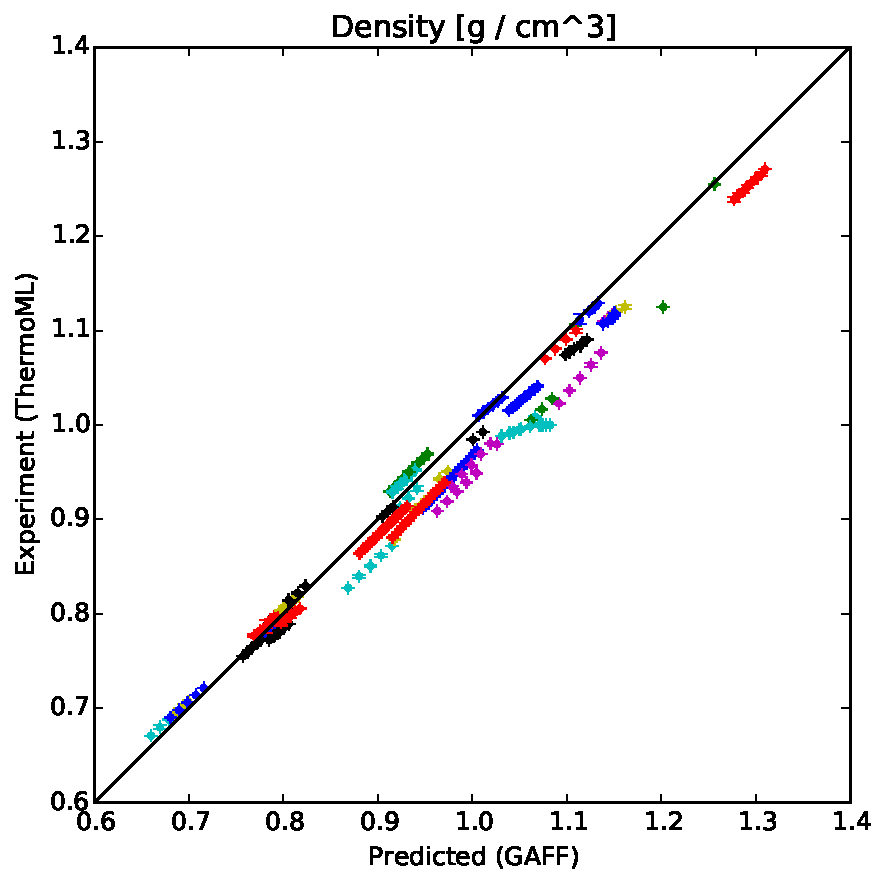
\includegraphics[width=9.5cm]{./figures/densities_thermoml.pdf}
}

\subfigure[]{
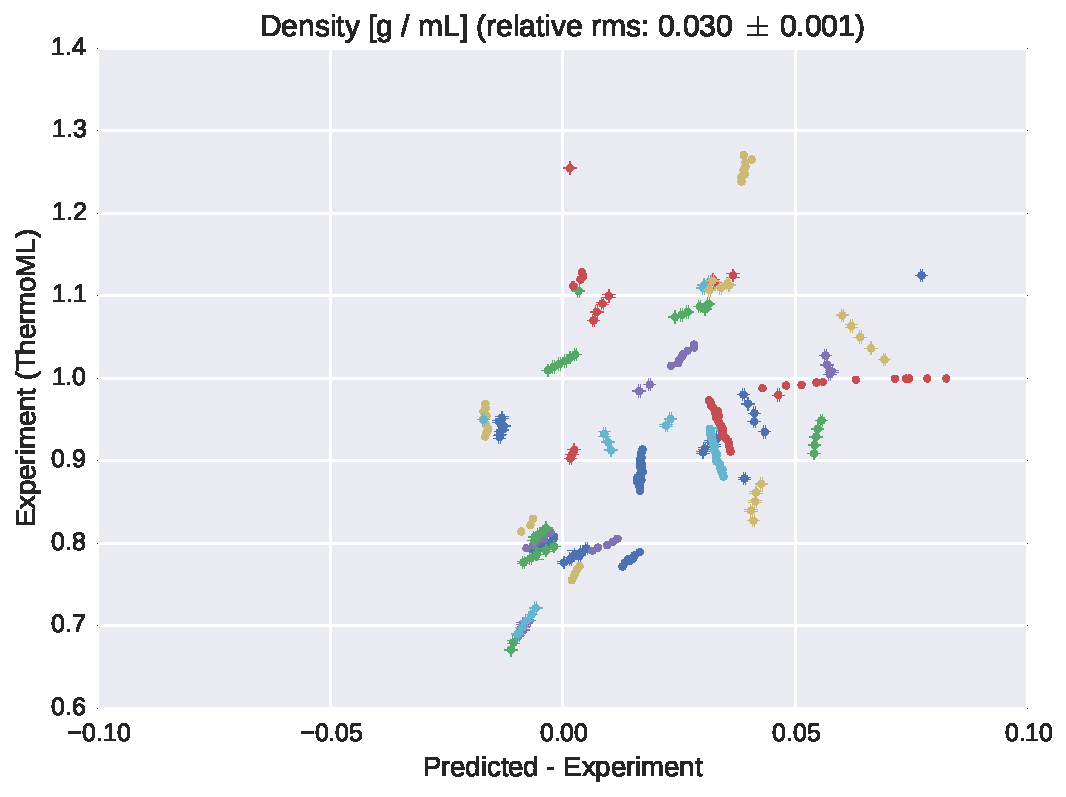
\includegraphics[width=9.5cm]{./figures/densities_differences_thermoml.pdf}
}

\caption{{\bf Comparison of liquid densities between experiment and simulation.}
(a).  Liquid density measurements extracted from ThermoML are compared against densities predicted using the GAFF / AM1-BCC small molecule fixed-charge forcefield.
Color groupings represent identical chemical species, although the color map repeats itself due to the large (45) number of unique compounds.
Plots of density versus temperature grouped by chemical species are available in Fig.~\ref{figure:AllDensities}.
Simulation error bars represent one standard error of the mean, with the number of effective (uncorrelated) samples estimated using pymbar.  
Experimental error bars indicate the standard deviation between independently reported measurements, when available, or author-reported standard deviations in ThermoML entries; for some measurements, neither uncertainty estimate is available.  
See Fig. \ref{figure:ErrorAnalysisDensity} for further discussion of error.  (b).  The same plot, but with the residual (predicted minus experiment) on the x axis.  Note that the error bars are all smaller than the symbols.  
}
\label{figure:Density}
\end{figure}

%%%%%%%%%%%%%%%%%%%%%%%%%%%%%%%%%%%%%%%%%%%%%%%%%%%%%%%%%%%%%%%%%%%%%%%%%%%%%%%%
% DIELECTRIC
%%%%%%%%%%%%%%%%%%%%%%%%%%%%%%%%%%%%%%%%%%%%%%%%%%%%%%%%%%%%%%%%%%%%%%%%%%%%%%%%

\subsubsection{Static dielectric constant}
\label{section:results:static-dielectric-constant}

{\bf Overall accuracy.}
As a measure of the dielectric response, the static dielectric constant of neat liquids provides a critical benchmark of the accuracy of electrostatic treatment in forcefield models.  
Discussing the accuracy in terms of the ability of GAFF/AM1-BCC to reproduce the static dielectric constant $\epsilon$ is not necessarily meaningful because of the way that the solvent dielectric $\epsilon$ enters into the Coulomb potential between two point charges separated by a distance $r$,
\begin{eqnarray}
U(r) = \frac{q_1 q_2}{\epsilon \, r} \propto \frac{1}{\epsilon} .
\end{eqnarray}
It is evident that $1/\epsilon$ is a much more meaningful quantity to compare than $\epsilon$ directly, as a 5\% error in $1/\epsilon$ will cause a 5\% error in the Coulomb potential between two point charges (assuming a uniform dielectric), while a 5\% error in $\epsilon$ will have a much more complex $\epsilon$-dependent effect on the Coulomb potential.
We therefore compare simulations against measurements in our ThermoML extract on the $1/\epsilon$ scale in Fig.~\ref{figure:Dielectric}.  

%{\color{red}[JDC: Can you provide any statistics about the overall error here, maybe also broken up into the error in high-dielectric and low-dielectric regimes?]}
% Done.  Added after the polarizability correction is introduced.  

{\bf GAFF/AM1-BCC systematically underestimates the dielectric constants of nonpolar liquids.}
Overall, we find the dielectric constants to be qualitatively reasonable, but with clear deviations from experiment, particularly for nonpolar liquids. 
This is not surprising given the complete neglect of electronic polarization which will be the dominant contribution for such liquids.
In particular, GAFF/AM1-BCC systematically underestimates the dielectric constants for nonpolar liquids, with the predictions of $\epsilon \approx 1.0 $ being substantially smaller than the measured $\epsilon \approx 2$.  
Because this deviation likely stems from the lack of an explicit treatment of electronic polarization, we used a simple empirical polarization model that computes the molecular electronic polarizability $\alpha$ as a sum of elemental atomic polarizability contributions~\cite{bosque2002polarizabilities}.

%\begin{equation} \label{eq:sales}
%\begin{split}
%\alpha/\textnormal{\AA} = 1.53 \, n_C + 0.17 \, n_H + 0.57 \, n_O + 1.05 \, n_N + 2.99 \, n_S \\ + 2.48 \, n_P + 0.22 \, n_F + 2.16 \, n_{Cl} + 3.29 \, n_{Br} + 5.45 \, n_I + 0.32 
%\end{split}
%\end{equation}

From the computed molecular electronic polarizability $\alpha$, an additive correction to the simulation-derived static dielectric constant accounting for the missing electronic polarizability can be computed~\cite{horn2004}
\begin{eqnarray}
\Delta \epsilon &=& 4 \pi N  \frac{\alpha}{\langle V \rangle} \label{equation:dielectric correction}
\end{eqnarray}
A similar polarization correction was used in the development of the TIP4P-Ew water model, where it had a minor effect~\cite{horn2004} because almost all the high static dielectric constant for water comes from the configurational response of its strong dipole.  
However, the missing polarizability is a dominant contribution to the static dielectric constant of nonpolar organic molecules;   
in the case of water, the empirical atomic polarizability model predicts a dielectric correction (to $\epsilon$) of 0.52, while 0.79 was used for the TIP4P-Ew model.  
Averaging this dielectric constant over all liquids in the present work leads to average polarizability corrections (to $\epsilon$) of $0.74 \pm 0.08$. 
Taking the dataset as a whole, we find that the relative error in uncorrected dielectric (to $\epsilon$) is on the order of $-0.34 \pm 0.02$, as compared to $-0.25 \pm 0.02$ for the corrected dielectric. 

%%%%%%%%%%%%%%%%%%%%%%%%%%%%%%%%%%%%%%%%%%%%%%%%%%%%%%%%%%%%%%%%%%%%%%%%%%%%%%%%
% FIGURE: DIELECTRIC COMPARISON
%%%%%%%%%%%%%%%%%%%%%%%%%%%%%%%%%%%%%%%%%%%%%%%%%%%%%%%%%%%%%%%%%%%%%%%%%%%%%%%%

\begin{figure}
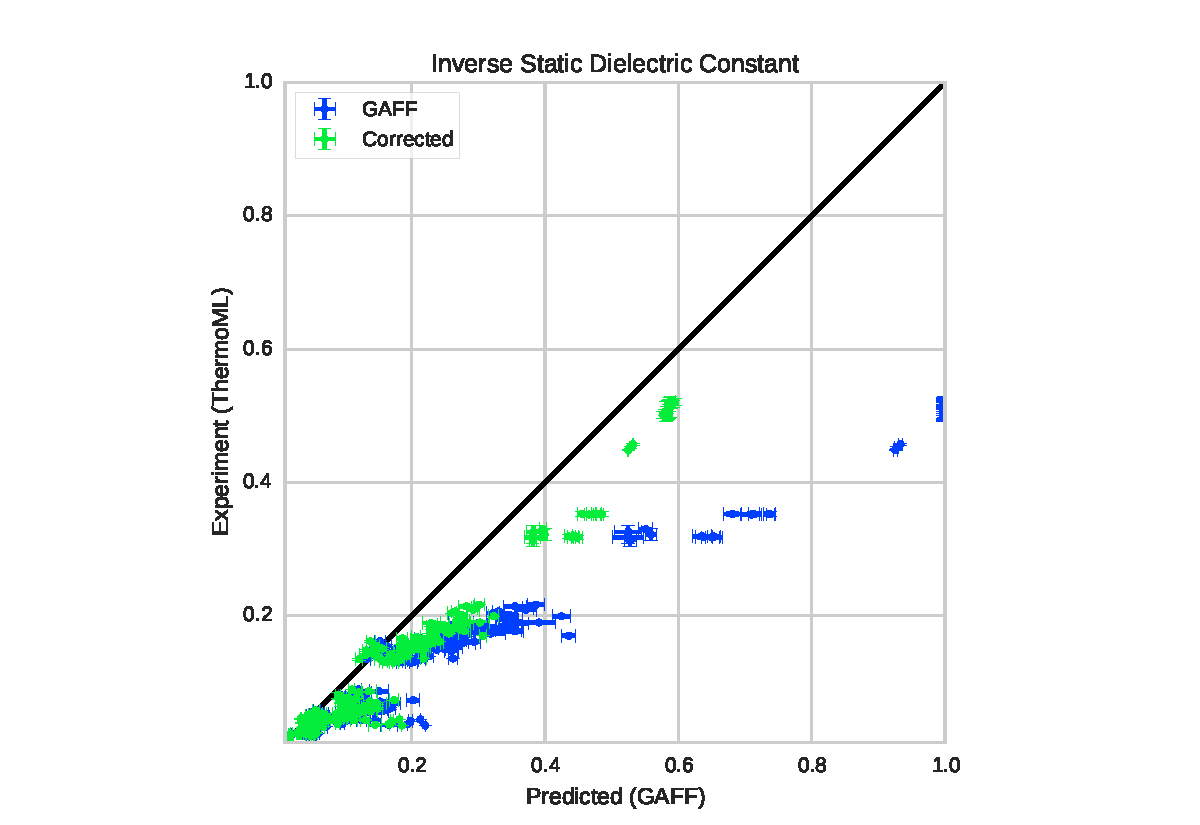
\includegraphics[width=\columnwidth]{./figures/dielectrics_thermoml.pdf}

\caption{{\bf Measured (ThermoML) versus predicted (GAFF / AM1-BCC) inverse static dielectrics (a).}
Simulation error bars represent one standard error of the mean.  
Experimental error bars indicate the larger of standard deviation between independently reported measurements and the authors reported standard deviations; for some measurements, neither uncertainty estimate is available.  
See Fig. \ref{figure:ErrorAnalysisDielectric} for further discussion of error.
See Section~\ref{section:results:static-dielectric-constant} for explanation of why inverse dielectric constant (rather than dielectric constant) is plotted. 
For nonpolar liquids, it is clear that the forcefield predicts electrostatic interactions that are substantially biased by missing polarizability.
Plots of dielectric constant versus temperature grouped by chemical species are available in Fig.~\ref{figure:AllDielectrics}.
}
\label{figure:Dielectric}
\end{figure}

%%%%%%%%%%%%%%%%%%%%%%%%%%%%%%%%%%%%%%%%%%%%%%%%%%%%%%%%%%%%%%%%%%%%%%%%%%%%%%%%
% DISCUSSION
%%%%%%%%%%%%%%%%%%%%%%%%%%%%%%%%%%%%%%%%%%%%%%%%%%%%%%%%%%%%%%%%%%%%%%%%%%%%%%%%

\section{Discussion}

\subsection{Mass densities}

Our simulations have indicated the presence of systematic density biases with magnitudes larger than the measurement error.  
Correcting these errors may be a low-hanging fruit for future forcefield refinements.
As an example of the feasibility of improved accuracy in densities, a recent three-point water model was able to recapitulate water density with errors of less than 0.005 g/cm$^{3}$ over the temperature range [280 K, 320 K] \cite{wang2014building}.
This improved accuracy in density prediction was obtained alongside accurate predictions of other experimental observables, including the static dielectric constant.  
We suspect that such accuracy might be obtainable for GAFF-like forcefields across some portion of chemical space.  
A key challenge for the field is to demarcate the fundamental limit of fixed-charge forcefields for predicting orthogonal classes of experimental observables.
For example, is it possible to achieve a relative density error of $10^{-4}$ without sacrificing accuracy of other properties such as enthalpies of vaporization?
In our opinion, the best way to answer such questions is to systematically build forcefields with the goal of predicting various properties to within their known experimental uncertainties, similar to what has been done for water \cite{horn2004, wang2014building}.


%%%%%%%%%%%%%%%%%%%%%%%%%%%%%%%%%%%%%%%%%%%%%%%%%%%%%%%%%%%%%%%%%%%%%%%%%%%%%%%%
% FITTING FORCEFIELDS TO DIELECTRIC CONSTANTS
%%%%%%%%%%%%%%%%%%%%%%%%%%%%%%%%%%%%%%%%%%%%%%%%%%%%%%%%%%%%%%%%%%%%%%%%%%%%%%%%

\subsection{Dielectric constants in forcefield parameterization}


A key feature of the static dielectric constant for a liquid is that, for forcefield purposes, it consists of two very different contributions, distinguished by the dependence on the fixed charges of the forcefield and dynamic motion of the molecule. 
One component, the electronic polarizability (which can be separately quantified through the high-frequency dielectric constant), arises from the almost-instantaneous electronic polarization in response to the external electric field.
Electronic polarizability contributes a small component, generally around $\epsilon = 2$, which can be dominant for non-polar liquids but is completely neglected by the non-polarizable forcefields in common use for biomolecular simulations. 

The other component arises from the dynamical response of the molecule through reorientation or conformational relaxation via nuclear motion.
For small polar liquids that lack significant internal degrees of freedom---such as water---reorientation of various molecular multipoles in response to the external electric field contributes the majority of the static dielectric constant. 
As a result, for polar liquids, we expect the parameterized atomic charges to play a major role in the static dielectric.  

Recent forcefield development has seen a resurgence of papers fitting dielectric constants during forcefield parameterization \cite{wang2014building, fennell2014fixed}.  
However, a number of authors have pointed out potential challenges in constructing self-consistent fixed-charge forcefields \cite{fennell2012simple, leontyev2014polarizable}.  


Interestingly, recent work by Dill and coworkers~\cite{fennell2012simple} observed that, for $\mathrm{CCl_4}$, reasonable choices of point charges are incapable of recapitulating the observed dielectric of $\epsilon = 2.2$, instead producing dielectric constants in the range of $1.0 \le \epsilon \le 1.05$.  
This behavior is quite general: fixed point charge forcefields will predict $\epsilon \approx 1$ for many nonpolar or symmetric molecules, but the measured dielectric constants are instead $\epsilon \approx 2$ (Fig.~\ref{figure:nonpolars}).  
While this behavior is well-known and results from missing physics of polarizability, we suspect it may have several profound consequences, which we discuss below.


%%%%%%%%%%%%%%%%%%%%%%%%%%%%%%%%%%%%%%%%%%%%%%%%%%%%%%%%%%%%%%%%%%%%%%%%%%%%%%%%
% FIGURE: Nonpolars
%%%%%%%%%%%%%%%%%%%%%%%%%%%%%%%%%%%%%%%%%%%%%%%%%%%%%%%%%%%%%%%%%%%%%%%%%%%%%%%%

\begin{figure}

\subfigure[]{
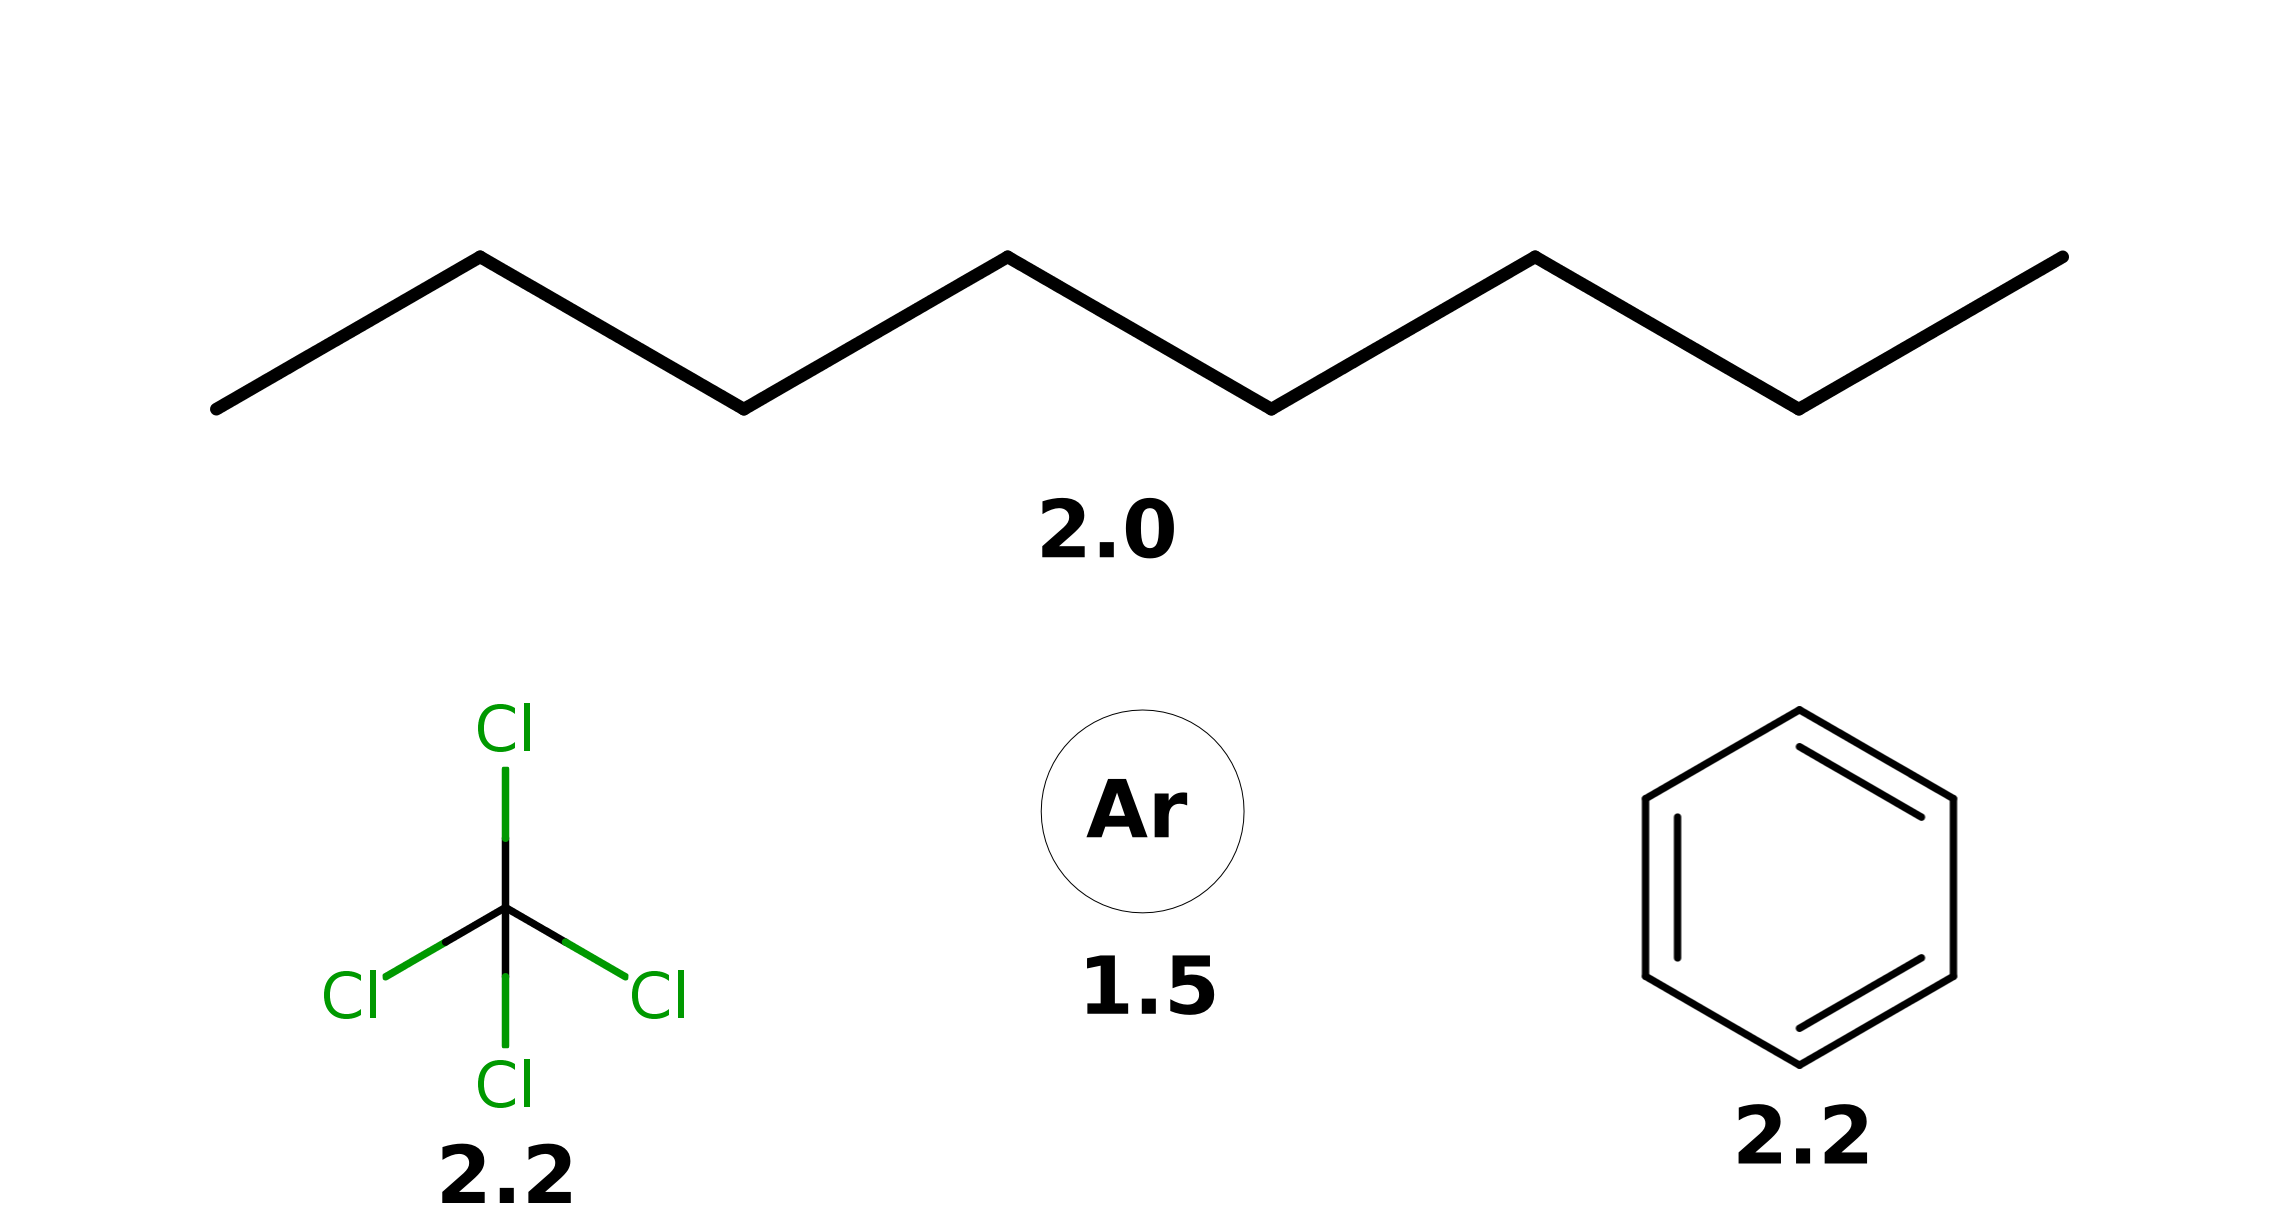
\includegraphics[width=\columnwidth]{./figures/molecules.png}
}

\noindent\rule{8cm}{0.4pt}
\subfigure[]{
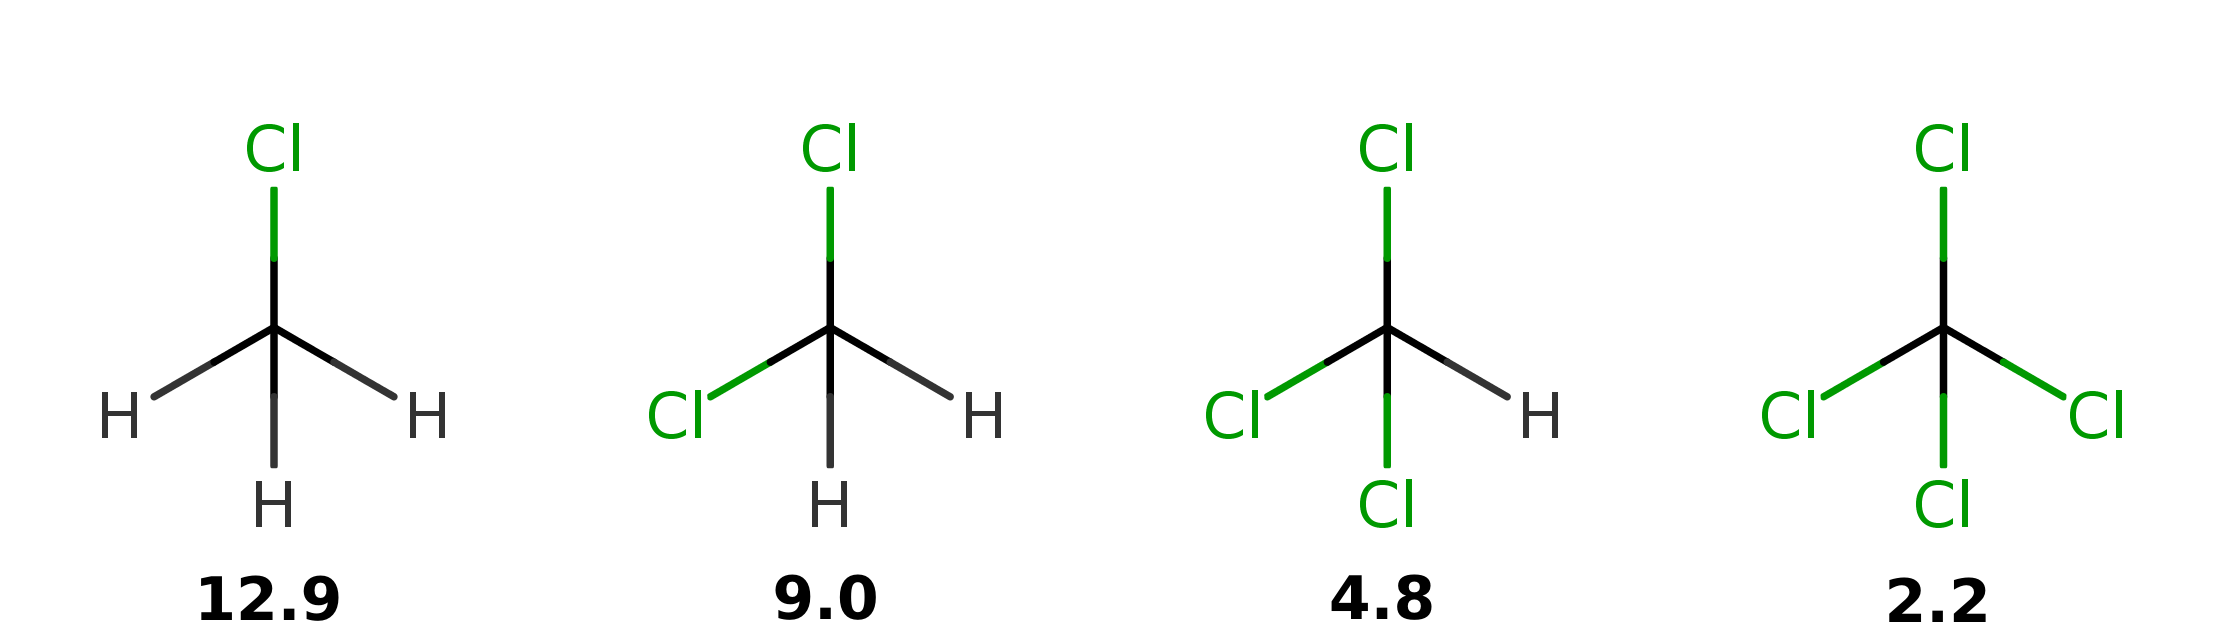
\includegraphics[width=\columnwidth]{./figures/chlorides.png}
}


\caption{{\bf Typical experimental static dielectric constants of some nonpolar compounds.}
(a). Measured static dielectric constants of various nonpolar or symmetric molecules~\cite{d1990dielectric, haynes2011crc}.  
Fixed-charge forcefields give $\epsilon \approx 1$ for each species; for example, we calculated $\epsilon = 1.0030 \pm 0.0002$ for octane.
(b).  A congeneric series of chloro-substituted methanes have static dielectric constants between 2 and 13.  
Reported dielectric constants are at near-ambient temperatures.  
}
\label{figure:nonpolars}

\end{figure}

%%%%%%%%%%%%%%%%%%%%%%%%%%%%%%%%%%%%%%%%%%%%%%%%%%%%%%%%%%%%%%%%%%%%%%%%%%%%%%%%

Suppose, for example, that one attempts to fit forcefield parameters to match the static dielectric constants of $\mathrm{CCl_4}$, $\mathrm{CHCl_3}$, $\mathrm{CH_2Cl_2}$, and $\mathrm{CH_3Cl}$.
In moving from the tetrahedrally-symmetric $\mathrm{CCl_4}$ to the asymmetric $\mathrm{CHCl_3}$, it suddenly becomes possible to achieve the observed dielectric constant of 4.8 by an appropriate choice of point charges.
However, the model for $\mathrm{CHCl_3}$ uses fixed point charges to account for \emph{both} the permanent dipole moment and the electronic polarizability, whereas the $\mathrm{CCl_4}$ model contains no treatment of polarizability.  
We hypothesize that this inconsistency in parameterization may lead to discontinuous jumps in physical properties in related molecular series, where symmetric molecules (e.g.,~benzene and $\mathrm{CCl_4}$) have qualitatively different properties than closely related asymmetric molecules (e.g.,~toluene and $\mathrm{CHCl_3}$).

How important is this effect?
We expect it to be important wherever we encounter the transfer of a polar molecule (such as a peptide, native ligand, or a pharmaceutical small molecule) from a polar environment (such as the cytosol, interstitial fluid, or blood) into a non-polar environment (such as a biological membrane or non-polar binding site of an enzyme or receptor). Thus we expect this to be implicated in biological processes ranging from ligand binding to absorption and distribution within the body. To understand this conceptually, consider the transfer of a polar small-molecule transfer from the non-polar interior of a lipid bilayer to the aqueous and hence very polar cytosol.

As a real-world example, we imagine that the missing atomic polarizability could be important in accurate transfer free energies involving low-dielectric solvents, such as the small-molecule transfer free energy from octanol or cyclohexane to water.  
The Onsager model for solvation of a dipole $\mu$ of radius $a$ gives us a way to estimate the magnitude of error introduced by making an error of $\Delta \epsilon$ in the static dielectric constant of a solvent.
The free energy of dipole solvation is given by this model as
\begin{equation} \label{eq:onsager}
\Delta G = -\frac{\mu^2}{a^3}\frac{\epsilon - 1}{2 \epsilon + 1}
\end{equation}
such that, for an error of $\Delta \epsilon$ departing from the true static dielectric constant $\epsilon$, we find the error in solvation is
\begin{equation} \label{equation:onsager-error}
\Delta \Delta G = -\frac{\mu^2}{a^3} \left[ \frac{(\epsilon+\Delta \epsilon) - 1}{2 (\epsilon+\Delta \epsilon) + 1} - \frac{\epsilon - 1}{2 \epsilon + 1} \right] 
\end{equation}
For example, the solvation of water ($a = 1.93$~\AA, $\mu = 2.2$~D) in a low dielectric medium such as tetrachloromethane or benzene ($\epsilon \sim 2.2$, but $\Delta \epsilon = -1.2$) gives an error of $\Delta \Delta G \sim -8$ kJ/mol (-2 kcal/mol).

{\bf Implications for transfer free energies.}
As another example, consider the transfer of small druglike molecules from a nonpolar solvent (such as cyclohexane) to water, a property often measured to indicate the expected degree of lipophilicity of a compound.
To estimate the magnitude of error expected, for each molecule in the FreeSolv database (as of 20 Feb 2015)~\cite{freesolv, freesolv_github}, we estimated the expected error in computed transfer free energies should GAFF/AM1-BCC be used to model the nonpolar solvent cyclohexane using the Onsager model (Eq.~\ref{equation:onsager-error}).
We took the cavity radius $a$ to be half the maximum interatomic distance and calculated $\mu = \sum_i q_i r_i$ using the provided mol2 coordinates and AM1-BCC charges.  
This calculation predicts a mean error of ($-3.8 \pm 0.3$) kJ / mol [($-0.91 \pm0.07$) kcal / mol] for the 643 molecules (where the standard error is computed from bootstrapping over FreeSolv compound measurements), 
suggesting that the missing atomic polarizabilty unrepresentable by fixed point charge forcefields could contribute substantially to errors in predicted transfer and solvation properties of druglike molecules.  
In other words, the use of a fixed-charge physics may lead to errors of $3.8$ kJ / mol in cyclohexane transfer free energies.  
We conjecture that this missing physics will be important in the upcoming (2015) SAMPL challenge \cite{newman2009practical}, which will examine transfer free energies in several low dielectric media. 

{\bf Utility in parameterization.}
Given their ease of measurement and direct connection to long-range electrostatic interactions, static dielectric constants have high potential utility as primary data for forcefield parameterization efforts.  
Although this will require the use of forcefields with explicit treatment of atomic polarizability, the inconsistency of fixed-charge models in low-dielectric media is sufficiently alarming to motivate further study of polarizable forcefields.  In particular, continuum methods~\cite{truchon2010using, truchon2009integrated, truchon2008accurate}, point dipole methods~\cite{Ponder2010, ren2004temperature}, and Drude methods~\cite{lamoureux2003modeling, anisimov2005determination} have been maturing rapidly.  Finding the optimal balance of accuracy and performance remains an open question; however, the use of experimentally-parameterized direct polarization methods~\cite{wang2013systematic} may provide polarizability physics at a cost not much greater than fixed charge forcefields.  
{\color{red}This is not to say that we suggest an immediate transition to polarizable force fields---the efficiency benefits and pervasiveness of fixed-charge models are important.  Furthermore, empirical corrections such as over-polarized charges \cite{fennell2012simple} and others \cite{leontyev2014polarizable} may provide the ability to model some low-dielectric behaviors at the cost of some transferability.  }


\subsection{ThermoML as a data source}

The present work has focused on the neat liquid density and dielectric measurements present in the ThermoML Archive~\cite{frenkel2006xml, frenkel2003thermoml, chirico2003thermoml} as a target for molecular dynamics forcefield validation.  
While liquid mass densities and static dielectric constants have already been widely used in forcefield work, several aspects of ThermoML make it a unique resource for the forcefield community.  
First, the aggregation, support, and dissemination of ThermoML datasets through the ThermoML Archive is supported by NIST, whose mission makes these tasks a long-term priority.  
Second, the ThermoML Archive is actively growing through partnerships with several journals, and new experimental measurements published in these journals are critically examined by the TRC and included in the archive.  
Finally, the files in the ThermoML Archive are portable and machine readable via a formal XML schema, allowing facile access to hundreds of thousands of measurements.  
Numerous additional physical properties contained in ThermoML---including activity coefficients, diffusion constants, boiling-point temperatures, critical pressures and densities, coefficients of expansion, speed-of-sound measurements, viscosities, excess molar enthalpies, heat capacities, and volumes---for neat phases and mixtures represent a rich dataset of high utility for forcefield validation and parameterization.

%%%%%%%%%%%%%%%%%%%%%%%%%%%%%%%%%%%%%%%%%%%%%%%%%%%%%%%%%%%%%%%%%%%%%%%%%%%%%%%%
% CONCLUSIONS
%%%%%%%%%%%%%%%%%%%%%%%%%%%%%%%%%%%%%%%%%%%%%%%%%%%%%%%%%%%%%%%%%%%%%%%%%%%%%%%%

\section{Conclusions}

High quality, machine-readable datasets of physicochemical measurements will be required for the construction of next-generation small molecule forcefields.  
Here we have discussed the NIST/TRC ThermoML archive as a growing source of physicochemical measurements that may be useful for the forcefield community.
From the NIST/TRC ThermoML archive, we selected a dataset of 246 ambient, neat liquid systems for which both densities and static dielectric constants are available.  
Using this dataset, we benchmarked GAFF/AM1-BCC, one of the most popular small molecule forcefields.
We find systematic biases in densities and particularly static dielectric constants.
Element-based empirical polarizabilty models are able to account for much of the systematic differences between GAFF/AM1-BCC and experiment.  
Non-polarizable forcefields may show unacceptable biases when predicting transfer and binding properties of non-polar environments such as binding cavities or membranes.  

\section{Supporting Information}

Five additional figures and one command line instruction are provided in the supporting information. This material is available free of charge via the Internet at \url{http://pubs.acs.org/}.

%%%%%%%%%%%%%%%%%%%%%%%%%%%%%%%%%%%%%%%%%%%%%%%%%%%%%%%%%%%%%%%%%%%%%%%%%%%%%%%%
% ACKNOWLEDGMENTS
%%%%%%%%%%%%%%%%%%%%%%%%%%%%%%%%%%%%%%%%%%%%%%%%%%%%%%%%%%%%%%%%%%%%%%%%%%%%%%%%

\section{Acknowledgements}

We thank Patrick B.~Grinaway (MSKCC), Vijay S.~Pande (Stanford University), Lee-Ping Wang (Stanford University), Peter Eastman (Stanford University), Robert McGibbon (Stanford University), Jason Swails (Rutgers University), David L.~Mobley (University of California, Irvine), Michael R. Shirts (University of Virginia), William C. Swope (IBM), Julia E. Rice (IBM), Hans Horn (IBM), Jed W. Pitera (IBM), and members of Chodera lab for helpful discussions.  
Support for JMB was provided by the Tri-Institutional Training Program in Computational Biology and Medicine (via NIH training grant 1T32GM083937).  
KAB was supported in part by Starr Foundation grant I8-A8-058.  
JDC and KAB acknowledge partial support from NIH grant P30 CA008748.  KAB, JMB, ASR, and JDC acknowledge the generous support of this research by the Sloan Kettering Institute.
The authors gratefully acknowledge OpenEye Scientific for generously providing their toolkit for use in noncommercial projects that generate results for the public domain.

%%%%%%%%%%%%%%%%%%%%%%%%%%%%%%%%%%%%%%%%%%%%%%%%%%%%%%%%%%%%%%%%%%%%%%%%%%%%%%%%
% DISCLAIMERS
%%%%%%%%%%%%%%%%%%%%%%%%%%%%%%%%%%%%%%%%%%%%%%%%%%%%%%%%%%%%%%%%%%%%%%%%%%%%%%%%

\section{Disclaimers}

This contribution of the National Institute of Standards and Technology (NIST) is not subject to copyright in the United States.  
Products or companies named here are cited only in the interest of complete technical description, and neither constitute nor imply endorsement by NIST or by the U.S.~government.  
Other products may be found to serve as well.

\clearpage


% Add figure label references for SI figures to allow cross referencing.


\setcounter{figure}{0}
\renewcommand{\thefigure}{S\arabic{figure}}  % Make figures say Fig. S1

\renewcommand{\figurename}{}
%\renewcommand{\thefigure}{}

\begin{figure}
\caption{}
\label{figure:timestep}
\end{figure}

\begin{figure}
\caption{}
\label{figure:ErrorAnalysisDensity}
\end{figure}

\begin{figure}
\caption{}
\label{figure:ErrorAnalysisDielectric}
\end{figure}

\begin{figure}
\caption{}
\label{figure:AllDensities}
\end{figure}

\begin{figure}
\caption{}
\label{figure:AllDielectrics}
\end{figure}


\bibliography{benchmark}

\clearpage

\section{TOC Figure}

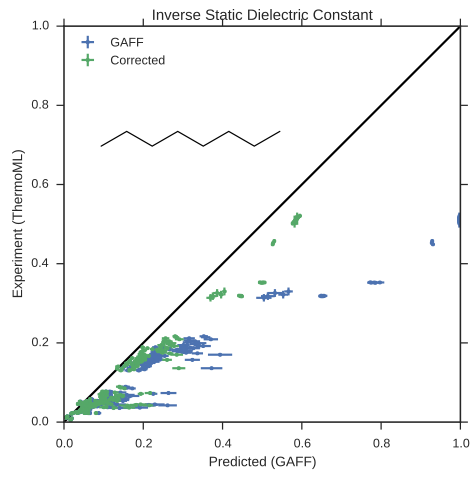
\includegraphics[width=\columnwidth]{./figures/scheme/toc_figure.png}


\end{document}
